\section{Faulty DNN Accelerator Analysis Platform and System Problems}
\label{sec:fault-analysis}
\subsection{Fault Analysis Platform}
To conduct system fault analysis on a realistic system, we build a fault 
analysis platform on Xilinx Zynq (ARM-FPGA) as shown in 
Figure \ref{fig:fault-analysis-overview}. It includes a full FPGA-based 
neural network acceleration system that has both a general purposed 
processor (ARM) and a DNN accelerator implemented on the FPGA. 
Typically, the processor sets up the neural network parameters through 
an AXI configuration port and allocates specific memory 
space for instruction/input/output/weight data. Then it can 
start the DNN accelerator. When the computing is done, DNN accelerator 
will notify the processor with interruption to collect the result from the 
shared DRAM. 

\begin{figure}
    \center{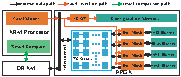
\includegraphics[width=0.99\linewidth]{system-overview}}
    \caption{Overview of the fault analysis system}
\vspace{-0.5em}
\label{fig:fault-analysis-overview}
\end{figure}

On top of the baseline FPGA-based neural network acceleration, 
we develop a configurable fault injection scheme. The injection data path 
is marked with the orange arrows and located on both the ARM processor and 
FPGA. On the arm processor part, we implement the fault models such as bit-flip, 
stuck-at-0, stuck-at-1, multiple-bit upset etc. and generate a set of bit errors 
based on a random fault distribution model. Then the errors are sent to 
the FPGA-based DNN accelerator from an AXI port. The errors are distributed to 
both FPGA configuration memory and the block RAM evenly based on the memory size.
Nevertheless, the error injection data paths to FPGA configuration memory 
and on-chip block RAM are quite different.

For FPGA configuration memory, we take advantage of Xilinx ICAP 
port \cite{UG953}, which allows user logic to access configuration 
memory, to inject errors. While Xilinx FPGA bitstream is organized 
as frames and each frame includes configuration bits of a block of 
FPGA, we randomly choose the frame and the number of bits for each 
bit error injection. The error can be located at any place of the 
FPGA configuration memory including the regions that are not utilized.
When the position of an error is determined, we read the whole frame 
out of the configuration memory via AXI port of AXI-HWICAP \cite{PG134}, 
change the victim bit in the frame, and write it back to the configuration 
memory \cite{UG470}. This can be done on the ARM processor either before the fault 
analysis or during the fault analysis. Thereby, the fault injection 
to FPGA configuration memory can either be performed with online 
manner or offline manner.

For the block RAM, we develop an error mask (Err. Mask) which can be 
added to a block RAM. The mask will not change the interface nor the 
pipelining of the original block RAM, but it has an AXI slace port
allowing ARM processor to flip a bit of any data in the block RAM 
during reading. Figure \ref{fig:error-mask} shows the design of the error mask.
Basically, it has a set of address and mask registers that can be configured 
using the attached AXI slave port. The addresses in the registers represent 
the position of errors to be injected while the corresponding masks 
keep the exact error bits. When there is a read request coming 
to the block RAM, the read address will be compared with all 
the addresses in the registers. when there is an address match, 
the data read from the block RAM will be XORed with the mask.
Then the result will be used as the output of the block RAM 
affected with injected errors. Since the registers in the error mask 
can either be configured runtime, the error injection to 
the block RAM can also be done in both an offline manner 
and an online manner.

\begin{figure}
    \center{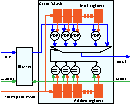
\includegraphics[width=0.8\linewidth]{error-mask}}
    \caption{Error mask for fault injection to buffers}
\vspace{-0.5em}
\label{fig:error-mask}
\end{figure}

Another important part of the fault analysis platform is the result 
collection and comparison. While the results of the neural networks 
running on the DNN accelerator are stored in the DRAM, it is 
Finally, we want to emphasize that the fault injection hardware is 
attached to the ARM processor with AXI slave port. With a 
driver, the AXI fault injection can be triggered in software running 
on the ARM processor.

\subsection{Consequences of faults in DNN accelerators}
\subsection{Fault model}
In our error injection design, the error injection to the 
configuration memory is global, regardless of whether the 
configuration block corresponding to the configuration bit 
is used. The injection of BRAM is designed to only inject 
errors into the BRAM used by user logic. In order to make 
the error injection as consistent as possible with the 
error generation under the radiation condition, we 
calculate the proportional relationship between the 
configuration memory and the block memory used.

Refer to Xilinx official documentations, the configuration 
Bitstream length of the XC7Z045 SoC used by the Zynq-7000 
SoC ZC706 Evaluation Board is 106,571,232 bits \cite{UG585}, which can 
be approximately regarded as the number of configured 
memory bits, and the available block memory is 20,090,880 
bits \cite{DS190}. After conversion, the accessible configuration memory 
accounted for about 84.14\%, while the block memory 
accounted for 15.86\%. In the NPU under test, the actual 
use of BRAM accounts for 30.43\% of the total bits, that is, 
4.83\% of the total bits of SRAM.

Based on the above calculations, we determined that the 
location where a single random error occurred would have an 
84.14\% chance of appearing in configuration memory and a 
4.83\% chance of appearing in actual used BRAM. When errors 
occur in these two areas, they can have an impact on the 
behavior and results of the system. In addition, the error 
will have an 11.03\% chance of appearing in unused BRAM, 
which will not have any impact on the system.

Before each Neural Network prediction, we randomly inject 
certain number of fixed upset errors into the system, which 
will persist in the process of Neural Network prediction 
until the end of prediction or timeout failure. After one 
prediction is performed, the errors in the system are 
recovered and the next random error injection and 
prediction is performed.


\subsection{Error Assessment}
We chose Neural Networks in four different application 
scenarios and try to analyze the differences of error 
tolerance in different application scenarios and networks. 
The four network applications include ResNet network for 
image classification, YOLO system for target detection, 
LSTM network for voice classification, and DCGAN network 
for image generation. We will evaluate their fault 
tolerance from accuracy and output consistency.

Neural Network accelerators injected with hardware errors 
may produce unexpected conditions. We define the system 
halt situation, which refers to a serious error in the 
system, or working improperly. such as unable to read and 
write registers, timeout, abnormal short runtime, etc. When 
the system halts, we need to reset the FPGA and restart the 
system. System halt situations are considered the result of 
errors in the evaluation of network accuracy and are listed 
separately in the output consistency.

Network accuracy refers to the overall accuracy of the 
network when performing corresponding tasks, such as the 
accuracy of 20,000 image recognition. When there are errors 
in the operation, the accuracy of the network will show a 
downward trend. For classification networks including 
ResNet and LSTM, top-5 accuracy is used to evaluate their 
accuracy, and for the YOLO system, mAP is adopted.

Output consistency is the difference between the result of 
running with errors injected and the result of normal 
running. We ran the corresponding data set when no errors 
are injected into each network at first, and defined the 
results as standard output. The results of Neural Networks 
prediction injected with errors are divided into two 
categories: result with deviation and result match. Result 
with deviation refers to system works properly with output 
differently from standard output. Result match means that 
the system works properly and the outputs are still 
standard output.

For the result with deviation case, we define its deviation 
quantitatively and further subdivide the result. Due to the 
different application functions of each network, the 
evaluation criteria of deviation are also different. For 
YOLO system, the result is the target detection bounding 
box, and when the detection result does not match the 
standard output in object type, it is defined as detection 
result error. When the result target type is consistent, 
the error is defined as the intersection area of the error 
output and the standard output divided by the area of the 
union. Target types not match for one single level, the two 
do not overlap with each other for one level, and then each 
20\% is divided into one level. For ResNet and LSTM, the 
outputs are top-5 labels. When the error output is not 
completely consistent with the standard output, the number 
of elements in the intersection of the two is taken, and 
divide the levels refer to the number. For DCGAN, we used 
the universal SSIM standard, and divided it into six levels 
according to the actual visual effects: 0~10\%, almost 
impossible to recognize; 10~20\%, barely visible; 20~50\%, 
with large deformation or distortion; 50~80\% with partial 
deformation or distortion; 80~90\%, small deformation or 
distortion can be seen; 90~100\%, almost no deformation or 
distortion is visible.
